
% Copyright 2013-2014 Tim Niemueller

\documentclass[a4paper]{article}
\usepackage{a4wide}
\usepackage{color}
\usepackage{tikz}
\usepackage{listings}
\usepackage{hyperref}
\usepackage{url}
\usepackage{array}
\usepackage{footmisc}
\usepackage[bitheight=6ex]{bytefield}

\usetikzlibrary{arrows,calc,through,backgrounds,shadows,decorations.pathreplacing}
\usetikzlibrary{positioning,decorations.text}
\newcommand{\refsec}[1]{Section~\ref{#1}}
\newcommand{\reffig}[1]{Figure~\ref{#1}}
\newcommand{\refdef}[1]{Definition~\ref{#1}}
\newcommand{\reflst}[1]{Listing~\ref{#1}}
%\newcommand{\reflst}[1]{Figure~\ref{#1}}

%% Mulberry Color for highlighting
\definecolor{Mulberry}{cmyk}{0.34,0.90,0,0.02}
\definecolor{BrickRed}{cmyk}{0,0.89,0.94,0.28}


\hypersetup{
  pdftitle      = {Referee Box for the RoboCup Logistics League},
  pdfauthor     = {Tim Niemueller},
  pdfkeywords   = {Robotics, RoboCup, LLSF, Referee Box},
  pdfsubject    = {Integration Manual 2014},
  %pdfpagemode   = {UseOutlines},        % PageWdth, FullScreen, None ...
  hidelinks    = true,          % true colored links, false colored boxes
%  linkcolor     = black,
%  citecolor     = black,
%  filecolor     = black,
%  urlcolor      = black,
%  backref       = false,
%  pagecolor     = black,         % link to other document pages
%  linktocpage,                  % linked page numbers instead of titles
%  menucolor   = blue,           % Acrobat menu item
%  pdfnewwindow= true,                %
%  pdfborder   = {0 0 0},             %
%  bookmarksopen=true,                %
%  bookmarksnumbered=true,            %
%  pdfcreator   = {pdflatex},
%  pdfproducer  = {latex-pdftex}
}

% required to make keywordsprefix for CLIPS working
% took me a while to figure it out, don't remove!
\lstset{language=Java}

\lstdefinelanguage{protobuf}{
  keywordsprefix=?,
  %keywordsprefix=\$,
  alsoletter={?=-<>*\$},
  keywordstyle=\color{Mulberry!90!black}\bfseries,
  keywords=[2]{package, message, extend, enum},
  keywordstyle=[2]\color{BrickRed!70!blue}\bfseries,
  keywords=[3]{float, double, int32 int64, uint32, uint64, sint32,
    sint64, fixed32, fixed64, sfixed32, sfixed64, bool, string, bytes},
  keywordstyle=[3]\color{darkgray}\bfseries,
  keywords=[4]{max},%
  keywordstyle=[4]\color{gray}\bfseries,
  keywords=[5]{required, optional, repeated},
  keywordstyle=[5]\color{red!60!black}\bfseries,
  %identifierstyle=\color{black},
  sensitive=false,
  comment=[l]{//},
  commentstyle=\color{purple}\ttfamily,
  stringstyle=\color{red}\ttfamily,
  morestring=[b]"
}


\lstdefinelanguage{cpp}{
  %keywordsprefix=?,
  %keywordsprefix=\$,
  %alsoletter={?=-<>*\$},
  keywordstyle=\color{Mulberry!90!black}\bfseries,
  keywords=[2]{typedef, struct, class, using, namespace, include,
    private, public},
  keywordstyle=[2]\color{BrickRed!70!blue}\bfseries,
  keywords=[3]{uint32_t, uint16_t, std::string, unsigned short, void},
  keywordstyle=[3]\color{darkgray}\bfseries,
  keywords=[4]{max},%
  keywordstyle=[4]\color{gray}\bfseries,
  %identifierstyle=\color{black},
  sensitive=false,
  comment=[l]{//},
  morecomment=[s]{/*}{*/},
  commentstyle=\color{purple}\ttfamily,
  stringstyle=\color{red}\ttfamily,
  morestring=[b]"
}

\lstdefinestyle{protobuf}
{
  language=protobuf,
  basicstyle=\footnotesize\ttfamily\vspace{0.2cm},
  breaklines=true,
  showstringspaces=false,
  %keywordstyle=\bfseries,
  %keywordstyle=\color{Mulberry},
  frame=lines,
  belowcaptionskip=8pt,
  emphstyle=\itshape,
  numbers=left,
  stepnumber=1,
  backgroundcolor=\color{blue!10},
  rulecolor=\color{blue!50},
  fillcolor=\color{blue!20},
  framexleftmargin=16pt,
  xleftmargin=16pt,
  %stringstyle=\color{BitterSweet},
  stringstyle=\color{BrickRed},
  commentstyle=\color{purple!50!black},
  escapechar=\%
  % emph={getup, servo, depends_skills},
  %emphstyle=\underbar,
  %numbers=left,
  %stepnumber=1,
  %%stringstyle=\ttfamily, % typewriter type for strings
}

\lstdefinestyle{cpp}
{
  language=cpp,
  basicstyle=\footnotesize\ttfamily\vspace{0.2cm},
  breaklines=true,
  showstringspaces=false,
  %keywordstyle=\bfseries,
  %keywordstyle=\color{Mulberry},
  frame=lines,
  belowcaptionskip=8pt,
  emphstyle=\itshape,
  numbers=left,
  stepnumber=1,
  backgroundcolor=\color{blue!10},
  rulecolor=\color{blue!50},
  fillcolor=\color{blue!20},
  framexleftmargin=16pt,
  xleftmargin=16pt,
  %stringstyle=\color{BitterSweet},
  stringstyle=\color{BrickRed},
  commentstyle=\color{purple!50!black}
  %escapechar=\%
  % emph={getup, servo, depends_skills},
  %emphstyle=\underbar,
  %numbers=left,
  %stepnumber=1,
  %%stringstyle=\ttfamily, % typewriter type for strings
}

\lstdefinestyle{small-protobuf}{
  style=protobuf,
  basicstyle=\ttfamily\footnotesize,
  numbersep=6pt,
}
\lstdefinestyle{really-small-protobuf}{
  style=protobuf,
  basicstyle=\ttfamily\scriptsize,
  numbersep=5pt,
}


\lstdefinestyle{really-small-cpp}{
  language=cpp,
  style=cpp,
  basicstyle=\ttfamily\scriptsize,
  numbersep=5pt,
}

\lstdefinestyle{really-small-protobuf-no-frame}{
  style=protobuf,
  basicstyle=\ttfamily\scriptsize,
  numbersep=5pt,
  frame=none,
  backgroundcolor=\color{white},
  framextopmargin=0pt,
  framexbottommargin=0pt
}

\lstdefinestyle{small-protobuf-no-frame}{
  style=protobuf,
  basicstyle=\ttfamily\footnotesize,
  numbersep=5pt,
  frame=none,
  backgroundcolor=\color{white},
  framextopmargin=0pt,
  framexbottommargin=0pt
}


\begin{document}
\title{\textbf{Referee Box for the RoboCup Logistics League}\\%
  \Large Integration Manual 2014}
\author{Tim Niemueller\\\href{mailto:niemueller@cs.rwth-aachen.de}{niemueller@kbsg.rwth-aachen.de}}
\maketitle

\section{Introduction}
\label{sec:intro}
Under the umbrella of RoboCup, in 2012 the first competition in the
\textit{Logistics League sponsored by Festo} (LLSF) took place. The
idea of this new RoboCup league is to simulate a production process
where an assembly robot has to bring goods to production places to
refine them step by step to a final product. A team of robots has to
explore which machine is producing/refining what semi-finished
products and produce as many products as possible.

Already at this early stage it became apparent, that just observing
the game and awarding points is complex. For the future, when
introducing more goods that can be processed, or when expecting more
robots operating concurrently, we need to consider options to automate
the evaluation of the game. This is the task of the referee
box~\cite{LLSF2013, LLSF2015}.

The Referee Box (refbox) controls and monitors the game to perform
this very evaluation. We have tried to make the refbox as autonomous
as possible. Textual and graphical user interfaces allow for human
instruction and supervision. This is in particular required in
unexpected situations (e.g. humans need to stop the game if a robot
catches fire) or where perceptual input is not available (a puck is
accidentally moved out of the area of a machine which is still waiting
for more goods). Several parts of the refbox were influenced by the
Fawkes Robot Software Framework~\cite{Fawkes} -- some libraries like
the configuration and logging facilities are simplified versions of
the Fawkes libraries -- and ROS~\cite{ROS}. The internally used CLIPS
environment is based on the Carologistics'~\cite{Carologistics-2013}
task coordination approach~\cite{CLIPS-Agent}.

This manual describes how to integrate a robot system with the refbox,
in particular the communication protocols involved. For detailed
information about system requirements to build and run the refbox as
well as configuration and usage instructions please refer to the
referee box website at \url{http://www.robocup-logistics.org/refbox}.

\section{Infrastructure}
\label{sec:infrastructure}
The refbox communicates with two different classes of entities, robots
and controllers. Any machine of a playing team is considered a
robot. Controllers are used by the human referees to interact with the
refbox, visualize its internal state, and give instructions to it.

All communication is handled using IPv4. There are two primary ways of
communication. First, controllers access the refbox using a TCP-based
stream communication protocol in a client-server fashion. Second,
robots communicate with the refbox using UDP-based broadcast protocol
in a peer-to-peer fashion.

Messages are defined and encoded using the Google protobuf library. It
provides easy to use, extensible, and widely compatible data exchange
structures. Messages are transmitted using a minimal protocol for
framing the serialized messages.

In the following we give a brief overview of Protobuf and how the
messages are defined. We then introduce the framing protocol and
how it is used to transmit messages. Afterwards we describe the
basic stream and broadcast communication modes and conclude with an
overview and example using the protobuf\_comm library which is part
of the refbox.

\subsection{Protocol Buffers (protobuf)}
Protocol
Buffers\footnote{\url{https://code.google.com/p/protobuf/}\label{fn:protobuf}}
(protobuf) offers a description language to define data exchange
formats which can be encoded and decoded very efficiently. The formats
are extensible and provide for basic data types, nesting, structure
re-use, efficient serialization and deserialization, variable-length
lists, and a compiler to create code for C++, Java, or Python to
access the data. In this document, we will only give a very brief
introduction and we refer to the protobuf website\footref{fn:protobuf}
for more detailed information.

Data structures are defined as messages containing fields, somewhat
similar to C/C++ data structures. Each field has a rule out of
\texttt{required}, \texttt{optional}, or \texttt{repeated}, a type,
a name, and a unique tag number. The rule defines if the field must
or can be present, or if it can be zero, one, or more values of the
given type. The type can be either one of a number of basic types,
or another message type. The tags must be unique within a message.
They are used to identify the fields when deserializing.

Structures in other files can be used by importing these files. See
for example BeaconSignal.proto as an example in
\refsec{sec:messages}.  After defining the messages in proto files,
they must be compiled to generate the actual code to use the data
structures. Protobuf comes with support for C++, Java, and Python
out of the box. For other languages third-party tools exist. The
code must then be compiled into a library or your application.

\subsection{Framing Protocol}

\begin{minipage}{\linewidth}
  \begin{minipage}[t]{.64\linewidth}
    \vspace{0pt}

    Once protobuf messages are serialized, they contain no information
    about the contained type or the length of the message. To use
    configurable encryption modes we need to indicate the used
    cipher. Therefore, to transmit them over the network a framing
    protocol is required. Our protocol consists of two parts, a
    protocol frame and a message header depicted on the right as a C
    struct. We will describe the headers and how messages are formed
    in more detail below, here is short overview.

    The first a structure carries protocol information like version,
    encryption cipher, and payload size. The second is the message
    header that indicates the protobuf message component and type type
    to allow for transmitting arbitrary messages over the same
    connection. Each message that is sent over the network is
    prepended by such headers.  After reading the frame header, the
    receiver must read as many bytes as indicated by
    \texttt{payload\_size} plus an additional IV header size if
    encryption is used and the cipher requires an IV (see below).
% As of
%    this writing, the \texttt{header\_version} will be set to 2. The
%    cipher will be either 0 (no encryption, used for stream, public
%    peer, and unencrypted team communication) or 2 (AES encryption
%    with 128 bits in cipher-block-chaining mode)
  \end{minipage}
  \hspace{.01\linewidth}
  \begin{minipage}[t]{.34\linewidth}
    \vspace{0pt}
\lstinputlisting[showlines,style=really-small-cpp,
firstline=74, lastline=87,
framexleftmargin=4pt, xleftmargin=4pt,numbers=none,
morekeywords={\$?ms},emph={merge,m-prio}]
{../../src/libs/protobuf_comm/frame_header.h}

\lstinputlisting[showlines,style=really-small-cpp,
firstline=99, lastline=104,
framexleftmargin=4pt, xleftmargin=4pt,numbers=none,
morekeywords={\$?ms},emph={merge,m-prio}]
{../../src/libs/protobuf_comm/frame_header.h}
  \end{minipage}
\end{minipage}

\smallskip

The message must be 4-byte-aligned, i.e. the size of the frame header
message structure sums up to exactly eight bytes when sent over the
network, the message header will be exactly four bytes. All contained
numbers must be encoded in network byte order (big endian, most
significant bit first). The numbers are encoded as 8
(\texttt{uint8\_t}), 16 (\texttt{uint16\_t}) or 32 bit
(\texttt{uint32\_t}) unsigned integers respectively.

When sending a message over the network, first the protobuf message is
serialized (to determine the payload size). Then the frame and message
headers are prepared with the appropriate component ID, message type,
and the payload size as just determined. Then the frame header is
sent, possibly followed by an encryption IV, again followed by the
message header and the the serialized message.

Note that for UDP packets, the data must be \emph{serialized into a
  single common buffer}. Otherwise the operating systems network stack
could split the transmission into multiple UDP messages. This is
invalid and cannot be decoded on the other end (UDP does not provide
for receiving in the correct order and packet correlation).

We will now describe the frame and message headers in detail and then
give examples for encrypted and unencrypted messages.

\subsubsection{Frame Header}
\paragraph{protocol version}
  The version of the protocol used. Currently this must be set to 2.
\paragraph{cipher}
  The cipher suite used. The acceptable values are listed in the
  following table.\\
  \smallskip\\
  \hspace*{4em}\begin{tabular}{l|l}
    \textbf{Value} & \textbf{Encryption mode}\\\hline
    0x00 & No encryption\\
    0x01 & AES 128 ECB\\
    0x02 & AES 128 CBC (requires 16 byte IV)\\
    0x03 & AES 256 ECB\\
    0x04 & AES 256 CBC (requires 16 byte IV)\\
  \end{tabular}
\paragraph{reserved}
  These bits are currently unused and must be set to zero.
\paragraph{payload size} Size in bytes of the following payload. This does
  include the message header and the serialized protobuf message. It
  does \emph{not} include an encryption IV header (if required by
  cipher). The payload size \emph{must} be encoded in network byte
  order (big-endian).

\subsubsection{Message Header}
\paragraph{component ID}
General ID, general addressee of message. For refbox message must be
set to 2000 (as encoded in the protobuf messages' COMP\_ID field of
the CompType enum. If you use the refbox framing protocol for your own
messages, choose a component ID different from the refbox ID. The
component ID \emph{must} be encoded in network byte order
(big-endian).
\paragraph{message type}
Numeric message ID of the specific message serialized in the
payload. Must be the ID encoded in the MSG\_TYPE field of the CompType
enum. The message type is specific to the component ID. Different
component IDs can have message of the same message type which are
unrelated. The message type \emph{must} be encoded in network byte
order (big-endian).

\subsubsection{Unencrypted Message}
\begin{figure}[htbp]
  \centering
  \hspace{5.3em}
  \begin{bytefield}{32}
    \bitheader{0,7-8,15-16,23-24,31} \\

    \begin{rightwordgroup}{frame \\ header}
      % We have to do the \parbox explicitly in the next line because
      % \hyperlink typesets its argument in horizontal mode.
      \bitbox{8}{\hyperlink{protocol-version}{protocol\\version = 2}} &
      \bitbox{8}{\hyperlink{cipher}{cipher = 0}} &
      \bitbox{8}{\hyperlink{reserved-2}{\vphantom{p}reserved = 0}} &
      \bitbox{8}{\hyperlink{reserved-3}{\vphantom{p}reserved = 0}} \\

      \wordbox{1}{\hyperlink{payload-size}{payload size}}
    \end{rightwordgroup} \\

    \begin{rightwordgroup}{message \\ header}
      \bitbox{16}{\hyperlink{component-id}{component ID}} &
      \bitbox{16}{\hyperlink{msg-type}{message type}}
    \end{rightwordgroup} \\

  \begin{rightwordgroup}{serialized \\ protobuf \\ message}
    \wordbox[lrt]{1}{%
      \parbox{0.6\width}{\centering (Protocol buffer message
        identified by component ID and message type)}} \\
    \skippedwords \\
    \wordbox[lrb]{1}{} 
  \end{rightwordgroup}

  \end{bytefield}
  \caption{Packet layout diagram for unencrypted message}
  \label{fig:unencrypted-packet}
\end{figure}
In \reffig{fig:unencrypted-packet} you see the byte layout for an
unencrypted data packet. Each row represents 4 byte of data. The
protocol buffer message is simply the buffer that is created by
serializing the message at hand. The component ID and message type
must be set as specified by the CompType enum in the message
definition, e.g. 2000 and 1 for a beacon signal message.

\subsubsection{Encrypted Message}
\begin{figure}[htbp]
  \centering
  \begin{bytefield}{32}
    \bitheader{0,7-8,15-16,23-24,31} \\

    \begin{rightwordgroup}{frame \\ header}
      \bitbox{8}{\hyperlink{protocol-version}{protocol\\version = 2}} &
      \bitbox{8}{\hyperlink{cipher}{cipher $> 0$\\\tiny 0x02 for AES-128-CBC}} &
      \bitbox{8}{\hyperlink{reserved-2}{\vphantom{p}reserved = 0}} &
      \bitbox{8}{\hyperlink{reserved-3}{\vphantom{p}reserved = 0}} \\
      
      \wordbox{1}{\hyperlink{payload-size}{payload size}}
    \end{rightwordgroup} \\

    \begin{rightwordgroup}{Crypto \\ IV}
      \wordbox{4}{\hyperlink{crypto-IV}{Initialization
          Vector\\(16 bytes for AES-128-CBC)}}
   \end{rightwordgroup} \\

    \begin{leftwordgroup}{encrypted\\part}
    \begin{rightwordgroup}{message \\ header}
      \bitbox{16}{\hyperlink{component-id}{component ID}} &
      \bitbox{16}{\hyperlink{msg-type}{message type}}
    \end{rightwordgroup} \\

    \begin{rightwordgroup}{serialized \\ protobuf \\ message}
      \wordbox[lrt]{1}{%
        \parbox{0.6\width}{\centering (Protocol buffer message
          identified by component ID and message type)}} \\
      \skippedwords \\
      \wordbox[lrb]{1}{} 
    \end{rightwordgroup}
    \end{leftwordgroup}
 
  \end{bytefield}
  \caption{Packet layout diagram for encrypted message}
  \label{fig:encrypted-packet}
\end{figure}
In \reffig{fig:encrypted-packet} you see the byte layout for an
encrypted data packet. It is similar to the unencrypted packet with
two key differences. First, the initialization vector is placed
between the frame and message headers. And second, the message header
and protobuf payload are encrypted.

\subsubsection{Encryption Modes}
The encryption currently implemented is intended to serve as a basic
protection layer in particular to prevent accidental transmission of
messages of the wrong team. For example, we do not insist on a
time stamp within the encrypted part of the messages which would aid
against replay attacks. This is done to avoid the need for time
synchronization between the robots and the refbox. This might be added
at a later point in time.

The framing protocol supports per-message encryption based on a
symmetric block cipher. For now, the supported encryption modes are
based on the AES\footnote{Advanced Encryption Standard,
  cf. \url{http://en.wikipedia.org/wiki/Advanced_Encryption_Standard}}
with either 128 or 256 bit key length in either electronic code book
(ECB) or cipher block chaining (CBC) mode. For the tournament, the
referee box will be configured to use the AES-128-CBC mode. This means
that there will be a 16 byte initialization vector (IV) which is used
to generate different encrypted messages for the same input (as long
as different IVs are provided).

The protobuf\_comm library handles this transparently for you. All you
need to do is to setup encryption on the team channel broadcast peer
(see below). Should you choose to create your own implementation,
please still take protobuf\_comm's BufferEncryptor and BufferDecryptor
classes for reference. The IV must be different for each transmitted
message.

\subsection{Communication Modes}
The refbox uses two communication modes. A TCP-connection-based
streaming protocol is used for communication between the refbox and
controllers like the shell or GUI. Teams may not use this mode to
contact the refbox. For such communication a UDP-based broadcast
protocol is employed.

Since the wifi is inherently unreliably, in particular during a
RoboCup competition, connections can be lost at any time. In
particular on a busy wireless network a TCP handshake can mean a
high performance penalty, or can even mean reliable communication
fails due to frequent re transmissions. Therefore, for
communication with the robots a UDP-based protocol was chosen. For
now, we use broadcasting to communicate the information to all
robots at once. In the future, this might be extended to Multicast.

To implement stream-based communication, we recommend to implement it
in such a way that always the frame header is read first, and only
afterwards the payload is read depending on the size given in the
header.

Broadcast-based communication is further split up into three
communication groups: public, team cyan, and team magenta. Generally,
teams should only send on their private team channel and listen to
both, the team and the public channel. The refbox will send its beacon
signal and the game state on the public channel, as it is the same for
both teams. Other messages like order information or exploration info
is sent per team. The exact assignment is specified in the message
descriptions.

For broadcast-based communication, make sure to build a complete
message buffer including the frame header and the serialized message,
and then send it in one go to avoid fragmentation. When reading,
create a sufficiently large buffer to read the full package at
once. Then read the frame header from the buffer and deserialize the
message.

\subsubsection{Communication Groups}
\begin{figure}
  \vspace{-3mm}
  \centering
    
  \tikzstyle{NW}=[outer sep=0,anchor=north west,minimum height=0.8cm]
  \tikzstyle{R}=[minimum width=3.2cm,minimum height=1cm,draw=black!50,fill=blue!20,text width=3cm]
  \tikzstyle{G}=[outer sep=0,anchor=south west, minimum width=4.8cm,
  minimum height=0.8cm, fill=green!20]


  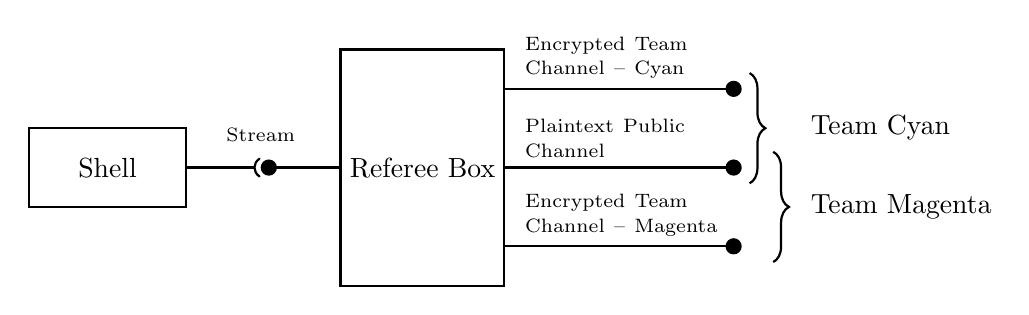
\begin{tikzpicture}[thick]

    \node (refbox)  [anchor=center,minimum width=2cm, minimum height=3cm,draw=black] at (0,0) {Referee Box};
    \node (shell)   [draw=black,minimum width=2cm, minimum height=1cm] at (-4,0) {Shell};
    \node (cyan)    [minimum width=2cm, minimum height=1cm,anchor=west] at (4.8, .5) {Team Cyan};
    \node (magenta) [minimum width=2cm, minimum height=1cm,anchor=west] at (4.8,-.5) {Team Magenta};

    \draw [>=*,->] (refbox.east |- 0,1) -- +(3,0) coordinate (cyan-end)
    node[above,pos=0.5,text width=2.5cm]{\scriptsize Encrypted Team\\[-.4em]
      Channel -- Cyan} ;
    
    \draw [>=*,->] (refbox.east |- 0,0) -- +(3,0)
    node[above,pos=0.5,text width=2.5cm]{\scriptsize Plaintext Public\\[-.4em]
      Channel};

    \draw [>=*,->] (refbox.east |- 0,-1) -- +(3,0) coordinate (magenta-end)
    node[above,pos=0.5,text width=2.5cm]{\scriptsize Encrypted Team\\[-.4em]
      Channel -- Magenta};

    \draw [decorate,decoration={brace,aspect=0.5,amplitude=2mm},thick] ($ (cyan-end) + (0.1,0.2) $) -- +(0,-1.4);
    \draw [decorate,decoration={brace,aspect=0.5,amplitude=2mm,mirror},thick] ($ (magenta-end) + (0.4,-.2) $) -- +(0,1.4);

    \draw [>=*,->] (refbox.west) -- +(-1,0) coordinate (shell-end);
    \draw [>=(,->,shorten >=2pt] (shell.east) -- +(1,0);
    \node [above of=shell-end,above=-8mm] {\scriptsize Stream};

  \end{tikzpicture}

  \caption{Communication channels and groups of the referee box}
  \label{fig:comm-groups}  
\vspace{-3mm}
\end{figure}
The refbox differentiates a total of four communication groups. These
are visualized in \reffig{fig:comm-groups}. Each team needs to open
two and only two broadcast peer communication channels during the
game.

\paragraph{stream}
The refbox accepts stream client connections on TCP port 4444. During
the tournament, connections will most likely only be allowed from the
local or selected hosts. Neither a robot nor any other team's device
may use the stream protocol to communicate with the refbox.

\paragraph{public}
The public broadcast channel is established on UDP port 4444. Teams
may only listen to this channel, but never send.

\paragraph{team channels}
There are two team channels on UDP ports 4441 (cyan) and 4442
(magenta). Each channel will be encrypted with a team-specific
encryption key that is created and provided to the teams at the
beginning of the tournament (and might be re-configured later should
the need arise). It is used for the private communication between the
teams and the referee box.

\subsubsection{Encryption Setup}
Encryption on the team channels should be configured only if the
refbox announced the respective team name for on of the two
colors. Teams may never send messages on a private team channel if it
is configured for a team different than their own.

The recommended flow for setting up encryption is like this:
\begin{itemize}
\item Listen to public channel for GameState messages
\item If the own team name is received as the cyan or magenta team
  name in the GameState message, setup encryption on the respective
  channel
\item Send messages on the team channel, never send messages on a
  channel of another team
\end{itemize}

\subsection{Example using protobuf\_comm}
The protobuf\_comm library provides an implementation of network
communication with protobuf messages using the framing protocol
described above for both communication modes. It is available as part
of the refbox source code\footnote{Instructions how to obtain the code
  at \url{http://trac.fawkesrobotics.org/wiki/LLSFRefBox/Install}} in
the \texttt{src/libs/protobuf\_comm} directory. The implementation
uses Boost Asio\footnote{\url{http://www.boost.org/libs/asio}} for the
asynchronous I/O implementation, and Boost
Signals2\footnote{\url{http://www.boost.org/libs/signals2/}} to
provide events that your code can connect to. The protobuf\_comm
library currently requires a compiler accepting code according to the
C++11 standard, e.g. GCC 4.6 or higher.

The library has three principal classes of interaction that you may or
may not use. First, the ProtobufStreamClient class implements a TCP
socket connection using the framing protocol to receive and transmit
messages from and to a ProtobufStreamServer, that is run in the
refbox. Second, the ProtobufBroadcastPeer implements peer-to-peer
communication over UDP using the framing protocol. Finally, the
MessageRegister is employed by both classes to register messages you
wish to react to. Messages types must be registered with the
message register so that the client or peer can know how to
deserialize incoming messages. Messages of an unknown type are
ignored.

The library uses the signal-slot event pattern to notify your code
about events such as being connected or disconnected, or receiving an
incoming message. This is built on top of Boost Signals2. Note that
this is incompatible with Boost.Signals. Signals2 was chosen because
it provides an increased thread-safety. The ProtobufStreamClient and
ProtobufBroadcastPeer run a concurrent thread to process incoming
data. So when a signal is issued, it happens in the context of the
receiving thread. For code that is not thread-safe, or that expects
events only from a particular thread (e.g. GUI applications using
Gtkmm or even text interfaces using ncurses), you need to implement a
dispatch pattern that will issue an event that is evaluated in that
main thread.

\begin{figure}
  \lstinputlisting[name=peer,showlines,style=really-small-cpp,
    firstline=37, lastline=114, numbers=left, stepnumber=5,
    numberfirstline=true,numberblanklines=true,
    framexleftmargin=16pt, xleftmargin=4pt]
    {../../src/examples/peer.cpp}
\vspace{-3mm}
\caption{Example program for a protobuf\_comm peer}
\label{fig:example-peer}
\end{figure}
\begin{figure}
  \lstinputlisting[name=client,showlines,style=really-small-cpp,
    firstline=37, lastline=95,numbers=left,stepnumber=5,
    framexleftmargin=16pt, xleftmargin=4pt]
    {../../src/examples/client.cpp}
\caption{Example program for a protobuf\_comm client}
\label{fig:example-client}
\end{figure}
In \reffig{fig:example-peer} you see the code for an example how to
use peer communication. You can also find the code in the
\texttt{src/examples} directory in the refbox source. You can adapt
the code and integrate it into your existing system. The full source
code can be compiled to a stand-alone program for testing. However,
you should integrate the code with your own main loop rather than
copying the stub from the example.

In the ExamplePeer class's constructor the peer is created (line
13--14) which also creates a new MessageRegister that will be used.
. In lines 13--14 the MessageRegister of the peer is retrieved, and
a single message type is registered. Note that no component ID or
message type are provided. They are retrieved from the CompType enum
field within the message specification (cf.~\refsec{sec:messages}). In
lines 16--20 the signals of the peer are connected to methods of the
ExamplePeer class. The events can be issued as soon as the signal is
connected. So make sure any required resource initialization has been
completed or is guarded when connecting the signals. The ExamplePeer's
\texttt{peer\_error} (line 30ff.) and \texttt{peer\_msg} (line 35ff.)
methods are called if a message reception failed or succeeded
respectively. Since the UDP communication is connection-less no
connected or disconnected signals exist. To detect that the refbox is
reachable listen to incoming BeaconSignal messages (see below). In the
\texttt{peer\_msg} method there are two ways to decide what message
has been received. You can either decide based on the component ID and
message type numbers (always both!), or you can use C++ Run-time Type
Information (RTTI). The latter is preferred and shown in the
example. It provides strong typing guarantees. As always, do not
forget to free the peer's resources by deleting it when no longer
required (destructor in line 24ff.).

In the ExampleClient class's constructor the client is created (line
12). In lines 14--15 the MessageRegister of the client is retrieved,
and a single message type is registered. Note that no component ID or
message type are provided. They are retrieved from the CompType enum
field within the message specification (cf.~\refsec{sec:messages}). In
lines 16--23 the signals of the client are connected to methods of the
ExampleClient class. The events can be issued as soon as the client is
connected. The \texttt{async\_connect} method of the client will
trigger connecting to the server, but it does not block. Make sure any
required resource initialization has been completed or is guarded when
connecting the client. Once the connection has been established, the
\texttt{connected} signal is issued and thus the ExampleClient's
\texttt{client\_connected} method (line~35ff.) is called. Likewise,
when the connection is lost the \texttt{client\_disconnected} method
(line~38ff.) is called with an error code indicating the reason of the
error. In the \texttt{client\_msg} method there are two ways to decide
what message has been received. You can either decide based on the
component ID and message type numbers (always both!), or you can use
C++ Run-time Type Information (RTTI). The latter is preferred and shown
in the example. It provides strong typing guarantees. As always, do
not forget to free the peer's resources by deleting it when no longer
required (destructor in line 29ff.).

\section{Messages}
\label{sec:messages}
In this section we describe the actual messages used for
communication. They are transmitted using the infrastructure described
above in accordance to the rules and regulations described in the LLSF
rule book.

Messages require a component ID and message type. The tuple must be
unique among all messages. The refbox uses the component ID 2000 for
all its messages. Messages are grouped in one file if they are
directly related. Within one file, one block of ten message type IDs
is used (with the principal messages BeaconSignal, AttentionMessage,
and VersionInfo being an exception).

The message types are encoded in the message proto files as a CompType
enum sub-type per message. The CompType must always be of the same
form, having a COMP\_ID and a MSG\_TYPE entry. The COMP\_ID is
assigned the component ID number, i.e. 2000 for the refbox. The
MSG\_TYPE is assigned the type identification number of the particular
message. It must be unique among all LLSF refbox messages. A message
type number may not be re-used once a message type is removed, as not
to confuse older peers expecting the old message type.

In the following, we give the protobuf specifications and description
of all message types currently used for the LLSF refbox
communication. The ``Via'' field describes what communication channel
is used to transmit the message, it can be either public broadcast
(P), team-private broadcast (T), or stream (S), or a combination
thereof. Many messages are sent at certain periods. These are given in
seconds time in between two sent messages, or event if it is sent on
particular events. Some broadcast messages feature a burst mode to
send a number of packets of the same content in short succession to
increase the chance of reaching the other peers. The ``Sent by'' and
``Sent to'' fields indicate the sender and receiver of a message. A
controller is the refbox GUI or shell to communicate to, not a team's
device. All proto files are in the \texttt{src/msgs} directory of the
refbox source code. Feel free to copy them to your own source code,
but in this case make sure to watch for updates to the messages and
integrate those changes\footnote{Register at
  \url{https://lists.kbsg.rwth-aachen.de/listinfo/llsf-refbox-commits}
  to the llsf-refbox-commits mailing list to be notified of any pushes
  to the refbox repository.}. The intention is to keep changes at a
minimum, especially when approaching a tournament. But in certain
situations may be necessary, e.g. to fix problems.

\bigskip

\newcommand{\msgspec}[6]{%
\hspace{-1.1\parindent}
\begin{minipage}{\linewidth}
  \begin{minipage}[t]{.48\linewidth}
    \vspace{0pt}
    \lstinputlisting[showlines,style=really-small-protobuf,
      firstline=37, escapechar=\%,%    %caption=,belowcaptionskip=2mm,
      framexleftmargin=4pt, xleftmargin=4pt,numbers=none,breakatwhitespace=true,
      morekeywords={\$?ms},emph={merge,m-prio}]
      {../../src/msgs/#1}
  \end{minipage}
  \hspace{.01\linewidth}
  \begin{minipage}[t]{.51\linewidth}
    \vspace{2pt}
    \small
    \begin{tabular}{>{\bfseries}ll>{\bfseries}ll}
      File:&\multicolumn{3}{p{.95\linewidth}}{%
        \texttt{#1}
      }\\[3pt]
      Groups:&#2&Period:&#3\\
      Sent by:&#4&Sent to:&#5\\[3pt]
      \multicolumn{4}{p{.95\linewidth}}{%
        #6
      }
    \end{tabular}
  \end{minipage}
\end{minipage}
}

\msgspec{AttentionMessage.proto}{S}{events}{refbox}{controller}%
{%
  An AttentionMessage is sent when a particular event requires human
  attention, e.g. if a late order puck must be placed or if
  communication to a robot is lost. If the team color is set the
  message should only be displayed if the color matches the monitored
  team (or indicate to which team it belongs to).
}

\msgspec{BeaconSignal.proto}{P, T}{1\,sec}{robots \& refbox}{any}%
{%
  The BeaconSignal is periodically sent to detect robots and the
  refbox on the network. If a robot is initially detected the time
  value is used to compare the clock offset (\emph{not} taking network
  delays into account). The controller may issue a warning if this is
  too large. The team and robot name are required to be able to
  diagnose possible connection problems. The refbox will set these
  fields to ``LLSF'' and ``RefBox'' respectively. The robots
  \emph{must} set the team color appropriately, only the refbox itself
  is allowed to not set it.

  \smallskip

  The referee box announces its presence on the public channel. The
  robots must use the team-private channel.

  \smallskip

  If a robot is not seen for more than 5\,seconds it is considered
  lost, and after 30\,seconds definitely lost.
  %, in which case it might
  %be removed from the field as per the dead robot rule.

  \smallskip

  We encourage teams to provide the position of the robot in the pose
  field to use it for visualization. Not only does it help the
  referee, but it will make the games more interesting to watch for
  visitors.
}

\msgspec{VersionInfo.proto}{S, P}{event}{refbox}{any}%
{%
  The VersionInfo message is sent to each newly connected stream
  client as the first message. Additionally, whenever a new peer is
  detected on the network, the version info is periodically sent 10
  times at a period of $0.5$\,sec. The information can be used to
  ensure compatibility and warn after future refbox upgrades.
}

\msgspec{Time.proto}{---}{---}{---}{---}%
{%
  This structure is used as a sub-message type within other messages
  and is never send by itself. It describes a point in time or a
  duration. What is sent depends on the contextual message.

  \smallskip

  A point in time is given relative to the Unix epoch in UTC time, for
  example using the \texttt{clock\_gettime()} POSIX API call, or using
  Boost's \texttt{posix\_time::universal\_time()} method.

  A duration is simply given as the number of seconds since the start
  and the number of nanoseconds since the start of the second.
}

\msgspec{Pose2D.proto}{---}{---}{---}{---}%
{%
  This structure is used as a sub-message type within other messages
  and is never send by itself. It describes a position and orientation
  on the 2D ground plane of the LLSF arena. The coordinate reference
  frame is aligned as described in the rule book.
}

\msgspec{Team.proto}{---}{---}{---}{---}%
{%
  This structure is used as a sub-message type within other messages
  and is never send by itself. It describes the team color, being
  either CYAN or MAGENTA (primary field side one or two respectively).
}

\msgspec{ExplorationInfo.proto}{P}{1\,sec}{refbox}{robots}%
{%
  This ExplorationInfo message is periodically sent during the
  exploration phase. It announces the mapping from type names to light
  signals and machine names referenced by field positions to the
  robots. There will be one entry per machine type in the signals
  list. The lights list in the ExplorationSignal sub-message will
  contain one entry per light color, even for signals which are
  off. The machines field contains one entry per machine to
  identify. The machines are referenced by a name bound to a specified
  position. Note that this name to position mapping might be different
  from the example in the rulebook.

  \smallskip
  Note the team color per machine. Only machines matching the team's
  color are to be reported.

  \medskip
  If one or more robots are presumably not receiving this message it
  is recommended to set the game state to PAUSED for some time. The
  ExplorationInfo message is continued to be sent in this state to
  allow the robot to catch up without jeopardizing the game.
}

\msgspec{GameInfo.proto}{S}{start}{refbox}{controller}%
{%
  Additional information about the game. This is sent on initial
  connection by the refbox to controllers. At the moment it contains a
  list of known teams that can be set by the controller as playing
  team.
}

\msgspec{GameState.proto}{S, P}{1\,sec}{refbox}{all}%
{%
  The GameState message is periodically sent via peer-to-peer to all
  robots as well as by client-server communication to connected
  controllers. The game time is restarted in the exploration and
  production phases, i.e. the time goes from 0 to 180 seconds in the
  exploration phase and from 0 to 900 seconds in the production phase.

  \medskip

  In the PRE\_GAME and POST\_GAME phases as well as in states other
  than RUNNING the robots must stand still immediately and all the
  time.

  \medskip

  The SetGameState and SetGamePhase messages can be used to request
  setting a new game state or phase respectively. They may only be
  sent by a controller. Be careful, setting a new phase will trigger
  re-initialization of that phase. To interrupt a game set the state
  to PAUSE, only modify the phase if you want to change
  irreversibly. It is illegal to send these messages from a robot. It
  will be detected by the refbox and considered a fraud attempt.
}

\msgspec{MachineInfo.proto}{S, T}{$0.25$\,sec}{refbox}{all}%
{%
  The MachineInfo message is sent periodically to controllers and
  robots (in production phase only) by the refbox. The message to
  \emph{controllers} includes static (inputs, output, name, type,
  pose) and dynamic information (pucks loaded into the machine area or
  placed under the RFID sensor, light signals, or whether it was
  correctly reported during the exploration phase) about all machines.
  The refbox may report only light signals that are on or
  blinking. Light color that are not mentioned should be considered to
  be off. It can be used for visually aligning machine representations
  with the actual position. The message is sent every $0.25$\,sec.

  The message broadcasted to \emph{robots} only includes name, type,
  input puck types, output puck type, and pose (as defined by the
  rulebook). It is sent only during the production phase over the
  team-private channel. At the beginning of the phase, the message is
  sent at a $0.5$\,sec period for 15\,sec. Afterwards the message is
  sent every 2\,sec.
 
  \medskip
  Both, the MachineInfo and Machine message types feature a team
  color. The team color on the latter is \emph{always} set. For the
  MachineInfo, the behavior differs between stream and broadcast
  messages. For stream messages, it is left out an a common
  MachineInfo message comprising \emph{all} machines of both teams is
  sent. For broadcasting, two messages are sent, one for each team. In
  these MachineInfo messages the team color will be set and only
  machines matching this color will be included.

  \medskip

  During the game the human referee at the refbox should take great
  care to notice any additionally connected controller (announced in
  the log window). No team computer or robot is allowed to connect to
  the refbox as particularly the machine state information allows for
  cheating.
}

\msgspec{MachineCommands.proto}{S}{event}{controller}{refbox}%
{%
  This protobuf file contains messages for specific instructions to
  the refbox, e.g. placing or loading a puck in the machine, or
  removing it. The commands can be also be used to write a game
  simulation that operates against a training refbox (without an
  actual PLC).
}

\msgspec{MachineReport.proto}{T}{$2$\,sec}{robots}{refbox}%
{%
  During the exploration phase robots announce recognized machines
  with the MachineReport message stating name and types. In each
  message, one or more machines can be reported. We suggest do always
  send all recognized machines to make sure that even in the case of
  packet losses, all machines are reported to the refbox
  eventually. The message should be send periodically, for example
  once every two seconds.

  \medskip

  Note that for each machine only the first report received is
  accepted and points are awarded according to the rule book and the
  correctness. It is not possible to correct a once given wrong
  report. Every subsequent repetition will be silently ignored. Also
  ensure that you send reports only for the appropriate team color or
  your report will be ignored. Sending machine reports for another
  team's machine with the other team's color is an offense.

  \medskip

  In the case of multiple robots there is \emph{no} need to
  synchronize their report to send one merged report. Instead each
  robot can report independently directly to the refbox. However,
  remember that only the first report for each machine is considered.

}

\msgspec{OrderInfo.proto}{S, T}{$5$\,sec}{refbox}{any}%
{%
  During the production phase the refbox periodically sends the
  current orders to all robots and controllers. Note that the list of
  orders in the OrderInfo message can and will change. If late orders
  get activated, new orders appear in the message. Also note the
  delivery period of orders. In a message, there will most likely be
  orders with an active delivery period, while others have already
  passed or are yet to come.

  \medskip

  Both, the OrderInfo and Order message types feature a team
  color. The team color on the latter is \emph{always} set. For the
  OrderInfo, the behavior differs between stream and broadcast
  messages. For stream messages, it is left out an a common OrderInfo
  message comprising \emph{all} orders of both teams is sent. For
  broadcasting, one messages per team-private channel is sent, one for
  each team. In these OrderInfo messages the team color will be set
  and only orders matching this color will be included.

  \medskip

  If a new order is posted, the refbox will go into a short time burst
  mode for a few seconds. During this time, it will send 10 messages
  at a period of $0.5$\,sec. Afterwards it continues with the normal
  period of $5$ seconds.
}

\msgspec{PuckInfo.proto}{S}{$1$\,sec}{refbox}{controllers}%
{%
  The PuckInfo message is sent periodically by the refbox to connected
  controllers. It contains state information about all pucks know to
  the refbox. The shell uses this information for the ``Pucks''
  section. Each puck has a unique ID and a current state.

  \medskip

  The pose information is optional and not currently provided. It may
  be used in the future with a camera-based tracking system.
}

\msgspec{RobotInfo.proto}{S, P}{$1$\,sec}{refbox}{controllers}%
{%
  The RobotInfo message is sent periodically by the refbox to
  connected controllers. It contains information about all robots
  known to the refbox. It reflects its belief gathered from processing
  BeaconSignal messages from the robots. It also contains a host name
  from where the BeaconSignal was received, for example to diagnose
  problems if a robot is lost.

  \medskip

  The pose information is optional. For teams which choose to provide
  this information in the BeaconSignal it is forwarded to the
  controller for visualization.
}

\msgspec{RobotCommands.proto}{S}{event}{controllers}{refbox}%
{%
  Commands related to robots that controllers can send to the
  refbox. Currently the only message allows to set the maintenance
  state of a particular robot of a particular team.
}

\section{Further Development}
\label{sec:dev}
The development of the refbox is an ongoing effort. While the basis
should be reasonably stable, there will be bugs that need to be fixed
and the refbox will have to be adapted to future rule changes. We
welcome comments and contributions when presented in a friendly
manner. There are some resources you can use to help us develop the
software and join the effort.

\begin{description}
\item[RoboCup Logistics mailing list] \hfill\\
  Please post questions and discuss issues and possible improvements
  on the RoboCup Logistics mailing list.\\
  \url{https://lists.kbsg.rwth-aachen.de/listinfo/robocup-logistics}
\item[Bug Reports] \hfill\\
  Bug reports should be submitted to the Fawkes Trac system for the
  ``LLSF RefBox'' component.\\
  \url{http://trac.fawkesrobotics.org/wiki/LLSFRefBox/ReportAProblem}
\item[Source Code] \hfill\\
  The source code is maintained as a git repository. See the
  installation instructions on how to get a copy. There is a web
  interface available to view the code and changes to it.\\
  \url{http://trac.fawkesrobotics.org/wiki/LLSFRefBox/Install}\\
  \url{http://git.fawkesrobotics.org/llsf-refbox.git}
\item[Licenses] \hfill\\
  Parts of the LLSF refbox are licensed under the 3-clause BSD
  license. Some parts, especially the ones originating from Fawkes,
  are released under the GNU General Public License Version 2 or later
  with special exceptions. See the header in the source code files for
  details.
\end{description}

%\nocite{*}
{\small
\bibliographystyle{unsrt}
\bibliography{llsf-refbox}
}

\end{document}
